\begin{figure}[tbp]
\centering
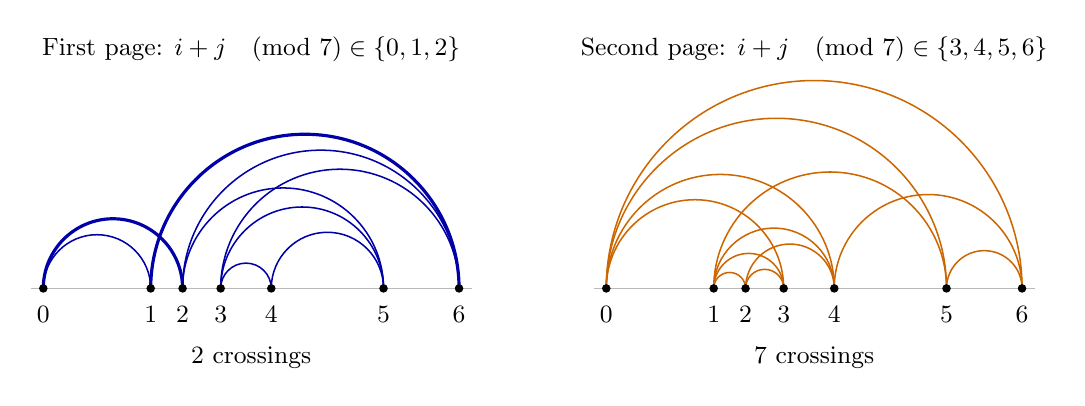
\begin{tikzpicture}[x=.88cm,y=.88cm,font=\small,
  spine/.style={draw=gray!55,line width=.35pt},
  first/.style={draw=blue!65!black,line width=.55pt},
  second/.style={draw=orange!80!black,line width=.55pt}]
  \def\positions{0/0,1/1.55,2/2.01,3/2.56,4/3.29,5/4.91,6/6}
  \begin{scope}
    \node[align=center] at (3,3.45)
      {First page: $i+j\pmod 7\in\{0,1,2\}$};
    \draw[spine] (-.18,0)--(6.18,0);
    \foreach \a/\b in {0/1.55,2.01/4.91,2.01/6,2.56/3.29,2.56/4.91,2.56/6,3.29/4.91} {
      \pgfmathsetmacro{\rad}{(\b-\a)/2}
      \draw[first] (\a,0) arc[start angle=180,end angle=0,radius=\rad];
    }
    \foreach \a/\b in {0/2.01,1.55/6} {
      \pgfmathsetmacro{\rad}{(\b-\a)/2}
      \draw[first,line width=1.15pt] (\a,0) arc[start angle=180,end angle=0,radius=\rad];
    }
    \foreach \i/\x in \positions {
      \fill (\x,0) circle (1.55pt);
      \node[below=3pt] at (\x,0) {$\i$};
    }
    \node at (3,-1.0) {$2$ crossings};
  \end{scope}
  \begin{scope}[xshift=7.15cm]
    \node[align=center] at (3,3.45)
      {Second page: $i+j\pmod 7\in\{3,4,5,6\}$};
    \draw[spine] (-.18,0)--(6.18,0);
    \foreach \a/\b in {0/2.56,0/3.29,0/4.91,0/6,1.55/2.01,1.55/2.56,1.55/3.29,1.55/4.91,2.01/2.56,2.01/3.29,3.29/6,4.91/6} {
      \pgfmathsetmacro{\rad}{(\b-\a)/2}
      \draw[second] (\a,0) arc[start angle=180,end angle=0,radius=\rad];
    }
    \foreach \i/\x in \positions {
      \fill (\x,0) circle (1.55pt);
      \node[below=3pt] at (\x,0) {$\i$};
    }
    \node at (3,-1.0) {$7$ crossings};
  \end{scope}
\end{tikzpicture}
\caption{The two-page construction for $K_7$. The pages are displayed
separately on the same labeled spine; reflect the second panel below
the spine to assemble the drawing. Page membership is determined by
the endpoint sum modulo $7$. The highlighted first-page edges $02$ and
$16$ cross because $0<1<2<6$. The displayed semicircles have $2$ and
$7$ distinct crossings.}
\label{fig:two-page}
\end{figure}
